\subsection*{Espejos de Lloyd}

\item 
\begin{minipage}[t][2.5cm]{0.4\textwidth}
En la figura se muestra una configuración para un interferómetro de Lloyd.
La fuente en \(S\) es puntual y monocromática está a una distancia \(a\) de un espejo plano de longitud \(D_1\).
La pantalla está ubicada a derecha del espejo a una distancia \(D_2\).
\end{minipage}
\begin{minipage}[c][1.5cm][t]{0.55\textwidth}
	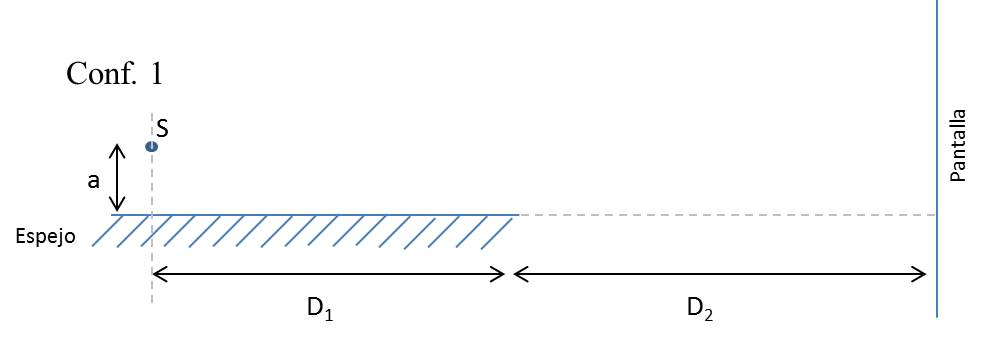
\includegraphics[width=\textwidth]{lloydEins}
\end{minipage}
\begin{enumerate}
	\item ¿Porqué es un interferómetro por división de frente?
	Halle la diferencia de camino óptico
	\item Defina el patrón de interferencia sobre la pantalla en función de los parámetros.
	¿Cuáles son las fuentes que interfieren?
	¿Cuál es su posición?
	¿Se producen desfasajes por reflexión?
	\item ¿Es posible observar franjas oscuras o brillantes en la pantalla a la altura del espejo?
	Determine la posición en la pantalla a partir de la cuál se observan franjas.
	\item Determine la intrerfranja si se ilumina con \(\lambda = \SI{600}{\angstrom}\), \(a = \SI{2}{\milli\metre}\), \(D_1 = \SI{25}{\centi\metre}\) y \(D_2 = \SI{25}{\centi\metre}\).
	\item Indique, sin necesidad de hacer cuentas, que diferencia presentan los patrones de interferencia en las pantallas las siguientes configuraciones respecto a la anterior.
\end{enumerate}
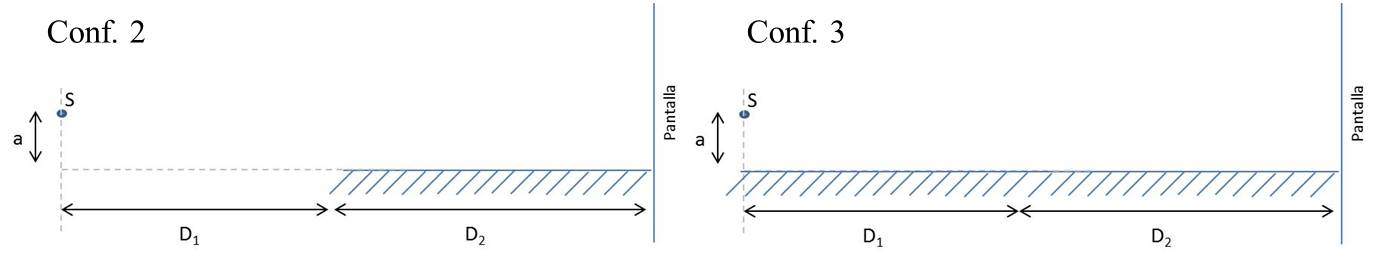
\includegraphics[width=0.95\textwidth]{lloydZwei}


\item (*) ¿Por qué motivo se puede concluir, en el experimento del espejos de Lloyd, que la luz reflejada ha sufrido un desfasaje de \ang{180;;}?
